\chapter*{Preface}\label{chapter:preface}
% c.f. https://tex.stackexchange.com/a/222961/152544
\addcontentsline{toc}{chapter}{\protect\numberline{}Preface}

The following is a summary of useful concepts in high energy particle physics.

\section{Units}\label{section:units}

\subsection{Natural Units}\label{subsection:natural_units}

The nature of high energy physics is to give descriptions of the phenomena and interactions that occur at energies that result in speeds that are close to the speed of light over very short time and distance scales.
Given this, it becomes readily apparent that SI units of measurement are somewhat cumbersome to cleanly explain calculations in, and a much more useful system of units would be to give calculation results relative to the scales that the phenomena occur at.
When measuring the speed of a relativistic particle it is more convenient to compare to the speed of light $\left(\text{such that }c=1\right)$ then to the number of meters per second.
Similarly, when measuring the momentum of a particle it is generally more useful to know the amount of its energy in the form of momentum compared to the amount in the form of its mass, resulting in expressing momentum in terms of energy.
This system of units is called ``Natural Units'' builds its measurements in terms of speed, angular momentum, and energy and is used extensively (if not almost exclusively) throughout high energy physics.
Quantities encountered routinely in high energy physics are given in Natural Units in \Cref{table:natural_units}.

\begin{table}[htpb]
 \centering
 \caption{Common quantities in particle physics given in both natural units and SI units.}
 \begin{tabular}{@{}llll@{}} \toprule
  Quantity         & Natural Units                 & Natural Units (dimensionful)            & SI Units                                              \\ \midrule
  Speed            & $1$                           & $c$                                     & $3.0\times 10^{8}~\textrm{m}/\textrm{s}$              \\
  Angular Momentum & $1$                           & $\hbar$                                 & $10^{34}~\textrm{m}^2 \,\textrm{kg}/\textrm{s}$       \\
  Energy           & \textrm{GeV}                  & \textrm{GeV}                            & $1.6\times 10^{-10}~\textrm{J}$                       \\
  Momentum         & \textrm{GeV}                  & $\textrm{GeV}/c$                        & $1\times 10^{-19}~\textrm{kg}\,\textrm{m}/\textrm{s}$ \\
  Mass             & \textrm{GeV}                  & $\textrm{GeV}/c^2$                      & $1.8\times 10^{-27}~\textrm{kg}$                      \\
  Time             & $1/\textrm{GeV}$              & $\hbar/\textrm{GeV}$                    & $6.6\time 10^{-25}~\textrm{s}$                        \\
  Length           & $1/\textrm{GeV}$              & $\hbar c/\textrm{GeV}$                  & $2\times 10^{-16}~\textrm{m}$                         \\
  Electric Charge  & $1$                           & $e/\sqrt{4\pi \alpha}$                  & $5.3\times 10^{-19}~\textrm{C}$                       \\
  Magnetic Field   & $\left(\textrm{GeV}\right)^2$ & $\left(\textrm{GeV}\right)^2/\hbar c^2$ & $5\times 10^{16}~\textrm{T}$                          \\
  \bottomrule
 \end{tabular}\label{table:natural_units}%
\end{table}


\subsection{Units of Luminosity}\label{subsection:luminosity_units}
In high energy physics a crucial quantity of interest is the luminosity (both instantaneous and integrated) delivered by the particle accelerator.
The instantaneous luminosity, $\mathscr{L}$, can be defined as the number of particles incident per unit area per unit time (generally taken to be seconds),
\begin{equation}
 \mathscr{L} = \frac{\text{number of particles}}{\text{unit area} \cdot \text{second}}.
 \label{eq:instantaneous_luminosity}
\end{equation}
In accelerator physics, the unit area is generally chosen to be $\textrm{cm}^2$, giving instantaneous luminosities units of $\textrm{cm}^{-2} \cdot \textrm{s}^{-1}$,
\[
 \left[\mathscr{L}\right] = \textrm{cm}^{-2} \cdot \textrm{s}^{-1}.
\]
However, experimental particle physicists prefer to use units of inverse barns for luminosities. A barn is defined as
\begin{equation}
 1~\textrm{barn} = 10^{-28}~\textrm{m}^2 = 10^{-24}~\textrm{cm}^2,
 \label{eq:barn_to_area}
\end{equation}
which is roughly the cross sectional area of an atomic nuclei.~\cite{web:history_physics_purdue,history:etymology_barn}\\

The context in which luminosity appears as being useful is in the form of an equation like
\begin{equation}
 N_{\textrm{events}} = \sigma_{\textrm{process}} \cdot \int \mathscr{L}\,dt
 \label{eq:events_from_luminosity}
\end{equation}
where:
\begin{itemize}
 \item $N_{\text{events}}$ is the number of events of a particular process that will be produced at the collider.
       This is what ends up hitting the detector.
 \item $\sigma_{\textrm{process}}$ is the cross section of the particular process to occur per interaction of colliding particles.
       At the \Gls{LHC} this would be the cross section per proton-proton interaction.
       This is a function of the fundamental physics that is available at the energy ranges being probed, and so is also a function of the collider's center of mass energy, $\sqrt{s}$.
       When written in an equation as such it is assumed that the cross section is also including the relevant branching ratios for the final state particles.
       That is, $\sigma\left(H \to b\bar{b}\,\right) = \sigma\left(pp \to H\right) \cdot \mathcal{BR}\left(H \to b\bar{b}\,\right)$.
 \item $L \equiv \int \mathscr{L}\,dt$ is the total luminosity integrated over time (the integrated luminosity).~\cite{Herr:941318}
       This is what is delivered by the particle accelerator.
\end{itemize}

\begin{table}[htpb]
 \centering
 \caption{Instantaneous luminosities at the LHC}
 \begin{tabular}{@{}ll@{}} \toprule
  Description                                                    & Units of $\textrm{cm}^{-2}\cdot\textrm{s}^{-1}$ \\ \midrule
  LHC Design Luminosity~\cite{Bruning:782076}                    & $10^{34}$                                       \\
  2017 ATLAS Trigger Menu Maximum~\cite{TWiki:MenuEvolution2017} & $2.0 \times 10^{34}$                            \\
  2017 Plan~\cite{Indico:MenuCoordination_2017Lumi}              & $1.7 \times 10^{34}$                            \\
  2017 Peak~\cite{TWiki:2017ATLASPeakLumi}                       & $20.9 \times 10^{33}$                           \\
  2018 Peak~\cite{TWiki:2018ATLASPeakLumi}                       & $21.0 \times 10^{33}$                           \\
  \bottomrule
 \end{tabular}\label{table:LHC_Luminosity_Goals}%
\end{table}

% Note to self: spacing in tables seems too large. See if can adjust with geometry package
\begin{table}[htpb]
 \centering
 \caption{Luminosity measurements in $\text{barns}^{-1}$}
 % \resizebox{\linewidth}{!}{%
 % \resizebox*{!}{\dimexpr\textheight-2\baselineskip\relax}{%
 \begin{tabular}{@{}lll@{}} \toprule
  Units                & Units of $\textrm{cm}^{-2}$ & Units of $\textrm{fb}^{-1}$ \\ \midrule
  $\textrm{barn}^{-1}$ & $10^{24}$                   & $10^{-15}$                  \\
  $\textrm{mb}^{-1}$   & $10^{27}$                   & $10^{-12}$                  \\
  $\mu\textrm{b}^{-1}$ & $10^{30}$                   & $10^{-9}$                   \\
  $\textrm{nb}^{-1}$   & $10^{33}$                   & $10^{-6}$                   \\
  $\textrm{pb}^{-1}$   & $10^{36}$                   & $10^{-3}$                   \\
  $\textrm{fb}^{-1}$   & $10^{39}$                   & $10^{0}$                    \\
  $\textrm{ab}^{-1}$   & $10^{42}$                   & $10^{3}$                    \\
  \bottomrule
 \end{tabular}\label{table:Luminosity}%
 % }
\end{table}

\section{Coordinates}\label{section:coordinates}

LHC coordinate systems\\

The LHC coordinate system, seen in \Cref{fig:LHC_coordinate_system}, is a rectangular coordinate system defined relative to the LHC ring and the LHC beamline.
At any point, the positive $x$ direction is defined as the direction that points radially inward to the center of the LHC ring.
The positive $y$ direction is then defined as pointing upwards --- towards the Earth's surface if one is at the beamline --- leaving the positive $z$ direction pointing along the beamline.\\

\begin{figure}[htbp]
 \centering
 \includegraphics{preface/LHC_coordinate_system.pdf}
 \caption{The LHC coordinate system as seen from the ATLAS detector.}
 \label{fig:LHC_coordinate_system}
\end{figure}

While the LHC coordinate system is Cartesian, the preferred coordinate system for describing LHC events is not.
As the ATLAS detector is arranged cylindrically outside the beamline of the LHC --- such that most of its detector components are transverse to the beamline --- the coordinate system that is used to describe events in ATLAS is characterized by a particle's transverse momentum, pseudorapidity, and polar angle: $\left(p_T, \eta, \theta\right)$.
The polar angle, $\theta$, is defined as the angle relative to the beam axis, and the azimuthal angle, $\phi$, is measured around the beam axis.\\

\Gls{Pseudorapidity} is defined as

\begin{equation}
 \eta = - \log \left(\tan \frac{\theta}{2}\right)
 \label{eq:pseudorapidity}
\end{equation}

to be a good approximation in the high energy regime of the \gls{rapidity} of a particle --- a measurement of the velocity of a particle longitudinal to the beam axis,

\begin{equation}
 y = \frac{1}{2} \log \left(\frac{E + p_{z}}{E - p_{z}}\right).
 \label{eq:rapidity}
\end{equation}

As the beam axis is defined as $\hat{\vec{z}}$, such that $p_{z} = \abs{\vec{p}} \cos\theta$, then it is seen that in the relativistic limit, $\abs{\vec{p}} \gg m$, the rapidity reduces to the pseudorapidity

\[
 \begin{split}
  y   &\approx \frac{1}{2} \log \left(\frac{p + p\cos\theta}{p - p\cos\theta}\right)\\
  &\approx \frac{1}{2} \log \left(\frac{2 \cos^{2} \frac{\theta}{2}}{2 \sin^{2} \frac{\theta}{2}}\right) \\
  &\approx - \log \left(\tan \frac{\theta}{2}\right) = \eta.
 \end{split}
\]

It is clear that the rapidity and the pseudorapidity are not \Glspl{Lorentz invariant}.
However, for a Lorentz \gls{boost} --- a Lorentz transformation without any rotations --- of speed $\beta$ along the beam axis, $\hat{\vec{z}}$,

\[
 \begin{pmatrix}
  E' \\
  p_{z}'
 \end{pmatrix}
 =
 \begin{pmatrix}%
  \gamma       & -\gamma\beta \\%
  -\gamma\beta & \gamma
 \end{pmatrix}%
 \begin{pmatrix}
  E \\
  p_{z}
 \end{pmatrix}\,,
\]

it is seen\footnote{Glossing over some algebra and hyperbolic trigonometric identities.} that the rapidity for a particle under the boost is the sum of the original rapidity and a constant of the boost
\[
 \begin{split}
  y'  &= \frac{1}{2} \log \left(\frac{E' + p_{z}'}{E' - p_{z}'}\right) \\
  &= \frac{1}{2} \log \left(\frac{E - \beta p_{z} + p_{z} - \beta E}{E - \beta p_{z} - p_{z} + \beta E}\right) \\
  &= \frac{1}{2} \log \left(\frac{E + p_{z}}{E - p_{z}}\right) + \frac{1}{2} \log \left(\frac{1 - \beta}{1 + \beta}\right) \\
  &= y - \tanh^{-1}\beta\,.
 \end{split}
\]

Thus, the \emph{difference in rapidities} between two particles is seen to be independent of the boost and so is a \Gls{Lorentz invariant}.
Defining the distance metric\footnote{$\Delta R$ is an angular distance in $\left(\eta, \phi\right)$ space, and can be thought of as a solid angle.} for two particles in $\left(\eta, \phi\right)$ space as
\begin{equation}
 \Delta R = \sqrt{\left(\Delta\eta\right)^{2} + \left(\Delta\phi\right)^{2}}
 \label{eq:DeltaR}
\end{equation}

it is seen that $\Delta R$ is by construction invariant to boosts along the beam axis.
As a result, \emph{translations} in $\eta$ of particles correspond to \glspl{boost} of the particles along the beamline.\\

For experiments at high energy colliders, the pseudorapidity offers a distinct advantage in the high energy limit as it only requires angular information while giving an excellent approximation to the rapidity.
Measuring both the energy and the full momentum for highly relativistic particles can be quite difficult, and as the differences between the rapidity and the pseudorapidity can quickly become very small, pseudorapidity is the favored measurement for experimental results.
Values of the pseudorapidity for values of the polar angle are summarized in \Cref{table:pseudorapidity_angles} and are plotted along with the form of \Cref{eq:rapidity} in \Cref{fig:pseudorapidity_angles}.

\begin{table}[htpb]
 \centering
 \caption{Polar angles relative to the LHC beam axis, $\theta$, and their corresponding pseudorapiditities, $\eta$.}
 \begin{tabular}{@{}cr@{}} \toprule
  Polar angle $(\theta)$ & Pseudorapidity $(\eta)$ \\ \midrule
  $\frac{\pi}{32}$       & $3.01335$               \\
  $\frac{\pi}{16}$       & $2.31779$               \\
  $\frac{\pi}{8}$        & $1.61489$               \\
  $\frac{\pi}{4}$        & $0.88137$               \\
  $\frac{\pi}{2}$        & $0$                     \\
  \bottomrule
 \end{tabular}\label{table:pseudorapidity_angles}%
\end{table}

\begin{figure}[htbp]
 \centering
 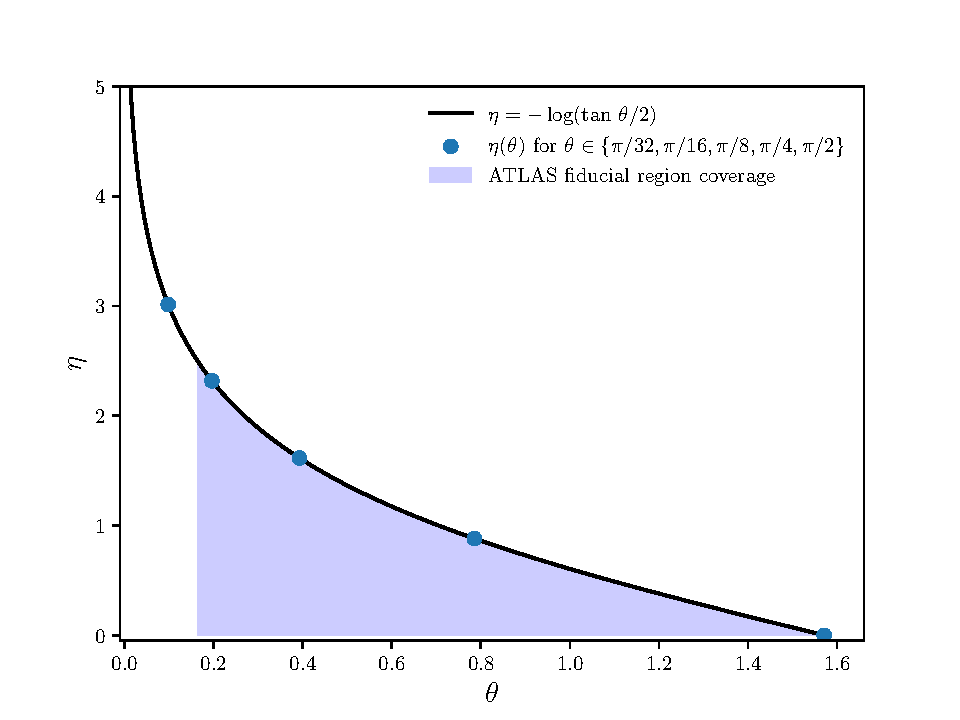
\includegraphics[width=0.8\linewidth]{preface/pseudorapidity.pdf}
 \caption{Pseudorapidity, $\eta = - \log \left(\tan \frac{\theta}{2}\right)$, as a function of the polar angle, $\theta$.
  The example markers are the points given in \Cref{table:pseudorapidity_angles}.
  The blue shaded region indicates the polar angle coverage up to $\eta = 2.5$, which is the end of the fiducial region coverage by the ATLAS inner detector.}
 \label{fig:pseudorapidity_angles}
\end{figure}

\section{Statistics}\label{section:statistics}

Statistics in particle physics

\section{Open Source Tools}\label{section:open_source}

This thesis and the researched described in it were made possible only through use of open source software.
The analysis was written in the open source languages \texttt{C++} and \texttt{Python} and made extensive use of the \texttt{ROOT} data analysis framework.
Similarly, parts of the analysis were conducted in Python and leveraged the SciPy ecosystem, most notably the NumPy and matplotlib libraries.
Additionally, the Keras library was used to interface with the TensorFlow machine learning framework for parts of the analysis.
The thesis itself was written in \LaTeXe, built using \texttt{latexmk} and \texttt{Make}, and versioned with Git.
Scientific research is built upon the open source community and tools, and this work would not have been made possible without it.
